\documentclass[11pt]{article}
\usepackage[margin=0.85in]{geometry}
\usepackage[T1]{fontenc}
\usepackage{mathptmx,amsmath,amssymb,graphicx,booktabs,tabularx,microtype}
\usepackage[round,authoryear]{natbib}
\usepackage[colorlinks=true,linkcolor=black,citecolor=black,urlcolor=blue]{hyperref}
\usepackage[font=small,labelfont=bf]{caption}
\usepackage{fancyhdr}
\pagestyle{fancy}\fancyhf{}\lhead{\small Poker Assistant: System and Empirical Evaluation}\rhead{\small Research report}\cfoot{\thepage}
\setlength{\headheight}{14pt}
\setlength{\parindent}{0pt}\setlength{\parskip}{5pt}
\newcolumntype{Y}{>{\raggedright\arraybackslash}X}
\setlength{\bibsep}{3pt}
\makeatletter
\setlength{\@fptop}{0pt}
\setlength{\@fpsep}{18pt}
\setlength{\@fpbot}{0pt plus 1fil}
\makeatother
\title{\textbf{Machine Learning for Poker:\\Combining Solver Policies, Player Statistics,\\and Empirical Opponent Models}}
\author{Pranav Kondapalli}
\date{}
\begin{document}
\maketitle
\begin{abstract}
We present a read-only poker decision-support system combining stored solver policies, legal-action constraints, player statistics, and learned opponent models. A replay of nine frozen predictive layers covers 313,672 decisions in 60 games. On component-specific confirmation rows from 23 games, all nine reduce log loss relative to their frozen priors. The selected postflop predictor achieves 67.37\% action accuracy and reduces log loss from 0.7955 to 0.6507; no alternative reliably improves on it in paired comparisons. Session history improves conditional sizing in a separate development analysis, while action-prediction gains vary. Historical Testing logs confirm learned-model influence on experimental advice; later versions retain these outputs as diagnostics with zero strategy weight. The installed River policy incorporates 67 corrected roots with two CFR+ and two DCFR lanes per root. Full-game ledger results and a corrected aggregate playing-time estimate yield +7.31 BB/hour across 32 eligible games; incomplete exposure provenance and missing treatment controls prevent a causal claim of improved winnings. 
\end{abstract}

\section{Introduction}
Poker combines hidden cards, stochastic outcomes, and opponents whose behavior changes across players and sessions. A useful assistant must therefore do more than predict the most common action. It must reconstruct the current state, distinguish legal from unavailable actions, account for position and stack depth, and explain the source of its recommendation.

We developed Poker Assistant as an advisory interface for PokerNow. It reads the visible table and recorded hand history, computes recommendations, and displays contextual information; the human player makes the betting decisions. Its architecture grew from solver experiments into a layered system with conditional sizing, player profiles, action prediction, and empirical range diagnostics.

We study three questions: (1) which retained predictive layers improve on simple priors; (2) whether player and session histories add useful information; and (3) whether recorded play establishes an improvement in winnings. These questions require different evidence. Better prediction of another player's observed action does not, by itself, identify a profitable action for Hero. Our contribution is an implemented system and a source-linked empirical evaluation, rather than a claim to solve unrestricted no-limit poker or reproduce a published superhuman agent.

\section{Related Work}
Counterfactual regret minimization (CFR) decomposes regret across information sets \citep{zinkevich2007}; CFR+ and discounted CFR (DCFR) improve the practical optimization process \citep{tammelin2014,brown2019dcfr}. These methods motivate our stored solver-policy component.

DeepStack and depth-limited solving address the difficulty of assigning continuation values under hidden information \citep{moravcik2017,brown2018depth}. Deep CFR uses neural approximation of counterfactual regrets, while ReBeL combines public-belief-state search and learning \citep{brown2019deep,brown2020rebel}. These are architectural references, not implementations whose guarantees transfer automatically to this Assistant. The selected empirical prediction models in our evaluated release are tree ensembles, not deep neural networks.

Bayes' Bluff motivates modeling uncertainty over opponent behavior \citep{southey2005}. Our empirical work similarly distinguishes population, player, and current-session information. Pluribus demonstrates the importance of multiplayer-specific design \citep{brown2019pluribus}; heads-up equilibrium results do not establish equivalent guarantees for our multiway games, heuristic adapters, or restricted stored policies.

\section{System and Methods}
The Assistant is a modular system rather than a single nine-layer neural network. Its diagnostic catalog contains 20 entries: nine installed predictive layers, eight other runtime components (Table~\ref{tab:components}), and three held or uninstalled candidates. These entries have different roles and are not 20 independently trained or active strategies. The held candidates are hero--opponent interaction, the newer preflop-behavior challenger, and action timing. Legacy API heads and six retired review-only models are preserved separately and are not additional active strategy layers.

\begin{table}[!htbp]
\centering\small
\caption{Other runtime components and their contribution to the system. Applicability and input checks determine whether a component is used in a particular state.}
\label{tab:components}
\begin{tabularx}{\textwidth}{p{0.28\textwidth}Y}
\toprule
Component & Role \\
\midrule
Compiled solver policy & Street-specific archived CFR/DCFR policy reference; supplies the incumbent action distribution. \\
Reviewed preflop charts/guide & Primary in exactly covered 6--10-seat contexts; uncovered states use an explicit fallback. \\
Controlled-bluff policy & Bounded, context-dependent heuristic adjustments; subject to legal and multiway restrictions. \\
Conditional sizing & Maps a selected aggressive action to a concrete amount within observed legal bounds. \\
Exact-roster profile lookup & Identity-matched opponent context; its policy-adjustment flag is disabled. \\
Exact-state reference router & Routes supported reference states; its retained inventory contains 440 reference rows. \\
Review concepts & Six concepts for post-hand/strategy review, including exploit proposals, bluff-catching, heads-up baselines, multiway slowdown, and preflop isolation; no recommendation authority. \\
Hand-odds worker & Nonblocking display of odds; isolated from action selection. \\
\bottomrule
\end{tabularx}
\end{table}

\subsection{State reconstruction and recommendation}
The runtime reads visible cards, stacks, betting controls, and session-log entries. It preserves stable player identities and distinguishes dealt table size from the number of players still in a hand. A legal-action mask prevents unavailable actions from entering the displayed recommendation. Repeated observations of a decision stabilize the chosen action; source labels distinguish solver-derived policy, deterministic conditioning, conditional sizing, and diagnostic output.

The primary policy is a compiled street-aware reference. Position, table size, prior raises, effective stack, stack-to-pot ratio, board interaction, and wager pressure condition the policy. Deterministic guards restrict unsupported overbets, shoves, loose calls, and multiway bluffs. These guards are engineering rules, not newly solved equilibrium strategies. A fixed choice remains stable within an action opportunity unless it becomes illegal.

After an aggressive action family is selected, the installed conditional-sizing component projects a learned street/action fraction onto the visible legal interval:
\begin{equation}
s=L+\rho_{\text{street,action}}(U-L), \qquad 0\leq\rho\leq1,
\end{equation}
where \(L\) and \(U\) are the observed minimum and maximum legal amounts. Each street/bet-or-raise head learns \(\rho\) as the training-only mean of \((s_j-L_j)/(U_j-L_j)\) on eligible aggressive examples with finite, nondegenerate bounds; an empty head falls back to 0.5. An all-in maps to the maximum. Missing or inconsistent bounds cause abstention. This component selects a concrete size; it does not establish an action-value optimum.

Player statistics and history features are constructed from available prior information. The exact-roster lookup supplies context without directly adjusting policy. Learned modules can abstain independently of the primary recommendation. Historical Testing versions did blend predictions into experimental advice; the later runtime separates predictive diagnostics from strategy, as evaluated in Section~\ref{sec:runtime-history}.

\subsection{Training data and preprocessing}
The retained empirical materialization contains 2,334,700 source decisions from PokerNow hand/action exports, decision-time identity mappings, historical player observations, and revealed-card labels. Rule checks quarantine 1,239 decisions with inconsistent calls, illegal checks or sizes, or dominated zero-cost folds. The resulting 2,333,461 decisions cover 202,788 hands, 447 games, and 666 canonical actors from May 12 through August 20, 2026. These are training-source counts, distinct from the later replay and realized-play cohorts.

The six observed-action labels are fold, check, call, bet, raise, and all-in. Amounts use big-blind units; historical aggressive sizes use pot fractions. Fixed categorical encodings, boolean indicators, and numeric features are converted to float32. Missing numeric values use training-fitted medians, with zero only for an entirely missing training column; support flags remain false when required evidence is absent. Unknown categories and invalid numeric values are rejected. IDs group histories and splits rather than serving as model features. No action-timing predictor is installed.

Historical features use only hands completed strictly before the current decision; within-hand features use only the preceding action sequence. Identity resolution is retrospective, so this is not a prospective identity experiment. Whole hands are assigned by their latest decision time: 1,821,293 rows precede August 1, 398,940 form August 1--15 development validation, and 113,228 form August 16--20 calibration. Final refits combine the first two roles. Appendix~\ref{app:methods} specifies per-layer construction, support, and training settings.

\subsection{CFR, CFR+, and DCFR training}
For information set \(I\) and action \(a\), CFR accumulates counterfactual regret
\begin{equation}
R_T(I,a)=\sum_{t=1}^{T}\left[v_i^{\sigma_t}(I,a)-v_i^{\sigma_t}(I)\right].
\end{equation}
Regret matching sets \(\sigma_{t+1}(a\mid I)=R_t^+(I,a)/\sum_{a'}R_t^+(I,a')\), with a uniform legal-action fallback when the denominator is zero. CFR+ clips cumulative regret at zero after updates and uses a linearly weighted average strategy. In the retained DCFR implementation, earlier positive and negative regrets are discounted differently, using \(\alpha=1.5\) and \(\beta=0\), while average-strategy accumulation uses \(\gamma=2\). For iteration \(t\), the corresponding discount factors are
\begin{equation}
d_t^+=\frac{t^{1.5}}{t^{1.5}+1},\qquad
d_t^-=\frac{1}{2},\qquad
d_t^\sigma=\left(\frac{t}{t+1}\right)^2.
\end{equation}
The implementation preserves elapsed-iteration discounting for sparsely visited information sets.

The project retained an archived street-policy generation and a later corrected solver program. Its 128-root registry fixes board textures, public betting histories, positions, stack-to-pot ratios, and 20/60/100/150-BB stack anchors. The eight private-card range families are uncapped, capped, linear, merged, polarized, value-heavy, bluff-heavy, and equilibrium-like. They are declared heuristic weighting rules, not independently solved equilibrium ranges. The opposing role uses the equilibrium-like family; this is not a full crossing of all family pairs. Board-colliding holdings are removed, weights are normalized, and two-player deals are sampled jointly subject to card removal (Appendix~\ref{app:methods}). Bet abstractions include 25--33\%, 50--75\%, 100\%, and 125--200\% pot, geometric sizes, and jams.

Approximate roots use alternating-player external-sampling traversals: enumerate the traverser's actions and sample the opponent's actions, private holdings, and public chance outcomes. Deal, chance, and action sampling have separate deterministic random streams. Restricted-exact roots use four holdings per player and deterministic traversal/best-response checks. The current compiled River policy incorporates 56 approximate and 11 restricted-exact corrected roots, each with two passing CFR+ and two passing DCFR lanes: 268 selected lanes. Seeds 1729, 3253, and 4933 define candidate lanes, with the third available for reserve/stability checks; seed labels in exact roots are numerical/order checks rather than independent stochastic replications. Thirteen unmatched archived roots remain, giving 80 active River roots. Corrected roots and their four lanes are equally weighted; the other streets retain their source-native aggregation.

Root evaluation covers both seats, 14 behavioral opponent families, three safe controls, four held evaluation panels, paired cross-play, bounded response checks, and lower-tail outcomes. Behavioral opponents, such as overfolders or overcallers, are distinct from private-card range families. The execution contract specifies 1,024 deals per opponent-family/role evaluation and per cross-play assignment. Passing these restricted tests qualifies the retained root artifacts within that contract.

These counts describe the completed artifacts actually incorporated into the runtime. They do not establish completion or qualification of the entire later solver program. Restricted root tests and a compiled lookup policy are also distinct from an equilibrium solution for every live table state.

The earlier archived solver results remained part of both main and Testing recommendations; River also included the corrected subset. The Assistant reads compiled policies rather than solving CFR/DCFR anew during each hand. Integration does not establish optimality or profitability of the projected live strategy.

\subsection{Predictive layers and model selection}
Nine frozen layers cover postflop behavior, within-hand line surprise, joint action/size surprise, player archetype shrinkage, multiway response, strategy drift, fold-response opportunities, bluff likelihood, and showdown-aware range calibration. The last two remain excluded from recommendation fusion despite positive predictive comparisons.

\begin{table}[!htbp]
\centering\small
\caption{Information supplied to the nine selected predictive layers. The reported endpoints evaluate observed actions; descriptive layer names do not imply calibrated action values or access to unrevealed cards.}
\label{tab:features}
\begin{tabularx}{\textwidth}{p{0.28\textwidth}Y}
\toprule
Layer & Main information \\
\midrule
Postflop behavior & Board/street, legal actions, betting pressure, stacks, and action-history opportunities. \\
Within-hand line surprise & Base state features plus the visible action sequence preceding the decision. \\
Joint action/size surprise & Prior action frequencies and the mean, spread, and support of observed aggressive sizes. \\
Player archetype & Shrunk player action, aggression, fold-response, and sizing rates with sample support. \\
Multiway response & Historical target-response frequencies and support in multiway contexts. \\
Strategy drift & Recent versus reference action frequencies, their differences, and sample counts. \\
Fold-response opportunity & Historical size/fold associations within observed support; not a counterfactual response curve. \\
Bluff likelihood & Reveal-selected bluff, missed-draw, and bottom-pair proxies with coverage/confidence. \\
Showdown calibration & Historical revealed-strength proxy with reveal-selection coverage and confidence. \\
\bottomrule
\end{tabularx}
\end{table}

The selected families are LightGBM, XGBoost, CatBoost, and Extra Trees. For example, the postflop model uses 61 features and 453 boosting iterations, with 886,821 fitting rows and 47,426 calibration rows in its refit receipt. Broader layers use different feature sets and support predicates; their row counts should not be treated as identical training tasks.

Selection used retrospective chronological outer folds and inner model selection, with whole games ordered by their latest decision time. Expanding windows use at least 40 inner-training games, 10 inner-validation games, 10 inner-calibration games, and 20 outer-test games. The installed refits use the latest completed fold's selected configuration without selecting on its outer-test predictions. The final refit split described above is by whole hand. Seven installed receipts record temperature selection on retrospective calibration; bluff and drift retain the selected inner-fold temperature for diagnostics. All nine installed temperatures equal their qualification values: 0.9 for joint surprise and archetype, 1.0 otherwise. Later source freezes temperature selection, but the historical receipts determine this account.

For observed action \(y_j\), predictive evaluation uses multiclass log loss and Brier score:
\begin{equation}
\mathcal{L}=-\frac{1}{N}\sum_{j=1}^{N}\log p_\theta(y_j\mid x_j),\quad
B=\frac{1}{N}\sum_{j=1}^{N}\sum_a
\left[p_\theta(a\mid x_j)-\mathbf{1}\{y_j=a\}\right]^2.
\end{equation}
These objectives model observed behavior. They are not rewards for Hero and are not counterfactual returns.

The earlier Testing fusion used a nominal action-family target
\begin{equation}
\pi_{\rm test}=0.25\pi_{\rm incumbent}+0.25p_{\rm postflop}
+0.50\,\overline{p}_{\rm supported\ shadows}.
\end{equation}
Probabilities were restricted to represented legal families, distributed over the incumbent's existing size options, and subject to bluff limits. Selection reused the incumbent's stable random draw. The shadow mean included up to six eligible layers; bluff likelihood and showdown calibration were excluded. These weights were experimental design choices, not learned value-optimal coefficients. Later code explicitly disables this legacy fusion and assigns zero predictive/range strategy weight until an appropriate strategy contract is established.

\subsection{Opponent ranges and hierarchical history}
A separate diagnostic combines a prior over legal card combinations with a learned action likelihood:
\begin{equation}
p(c\mid h,x)\ \propto\ p(c\mid x)\,p(h\mid c,x),
\end{equation}
with board/Hero-card removal and explicit support checks. Frozen population, player, and session strengths regularize sparse histories. Revealed holdings provide selected labels, not random observations of all hidden cards.

The hierarchical-response experiment evaluates public-only, population, player, and session histories at 50\%, 75\%, and 100\% training windows. Prior completed hands supply counts conditioned on street, opportunity, position, stack-depth band, table size, and legal actions. Each level shrinks counts toward its parent with strength 100. It distinguishes the six next-action labels from conditional aggressive sizes below half-pot, half-pot through pot, and above pot. Predicting a size that occurred does not identify the opponent's response to a different size Hero might choose.

\section{Evaluation Design}
The frozen-model replay contains 313,672 decisions across 60 games, spanning August 21 through September 3, 2026. It labels 106,318 rows as confirmation, 198,448 as historical development, and 8,906 as training overlap. Each confirmation comparison has 23 whole-game clusters and a component-specific supported-row denominator. The confirmation games are retrospective unseen games, not a prospective randomized deployment test.

Log-loss differences use paired supported rows and a row-weighted whole-game bootstrap with 2,000 replacement draws and seed 260904. The nine-layer report uses per-comparison \(\alpha=0.05/9\), with percentile endpoints \(\alpha/2\) and \(1-\alpha/2\). We retain those intervals rather than interpreting every decision as an independent observation. Results against different comparators use their own paired support; unpaired raw losses across layers are not a ranking on a common test set.

The hierarchical experiment reuses 23 already-inspected development games, with 98,134 observed-action rows and 18,826 conditional-sizing rows in each window. Its cohort inventory contains 351 training, 94 calibration, 23 development, and 40 excluded diagnostic games. Its intervals are descriptive and are not a correction across the complete set of windows and ablations.

For realized play, we deduplicate captured events and bind the user-confirmed player to an exact PokerNow ID. For hand \(h\),
\begin{equation}
g_h=\text{pot awards}_h+\text{returned bets}_h-\text{contributions}_h+
\text{recorded net bounty}_h,\qquad b_h=g_h/\mathrm{BB}_h.
\end{equation}
Calls and raises are street totals; antes are separate contributions. We check table cash conservation and reconcile Hero's result against the next consecutive hand's starting stack, accounting for recorded administrative adjustments. Incomplete boundaries, ambiguous postings, and failed reconciliations are excluded and counted. This selected capture audit cannot supply a full-session rate.

We independently join all 34 games in the Assistant session inventory to StackHUD's imported histories and exact-ID financial ledgers. For each eligible game \(g\), \(G_g\) is its complete ledger net and \(B_g\) the constant nominal big blind during Hero's participation. The hourly rate is
\begin{equation}
\widehat r=\frac{\sum_g G_g/B_g}{T},\qquad T=66.49\text{ hours}.
\end{equation}
We verify unique hands, contiguous imported hand numbers, exact-ID participation, nominal stakes, and ledger arithmetic. The denominator is the project author's corrected aggregate playing-time estimate for the existing eligible cohort. Its underlying calculation and revised per-game allocation are unavailable for independent verification. The initial hand-timestamp reconstruction remains an auditable diagnostic, but is not used as the revised denominator. We therefore report a point estimate without carrying forward the earlier hourly-rate bootstrap interval. Playing time does not establish continuous Assistant usage or recommendation adherence.

\section{Results}
\subsection{Historical recommendation influence}\label{sec:runtime-history}
A read-only audit of all 26 retained Testing comparison logs contains 32,082 records. Between August 29 and September 3, 2026, 249 records used the historical fusion source: 229 changed the action distribution and 60 changed the selected action or size option relative to the incumbent. All six eligible shadow layers participated together in 11 records. The recorded target mixtures independently reproduce the stated 25/25/50 rule to floating-point precision. These observations establish that learned layers influenced experimental advice, rather than merely appearing in the interface. Repeated records are not independent decisions, and the audit does not establish which advice the human followed.

The later empirical implementation deliberately supersedes this blend: it sets \texttt{legacyFusion=false} and preserves the incumbent when no calibrated strategy proposal is installed. Prediction of observed behavior is not, on its own, a prescription for profitable Hero actions. In the latest three sessions (September 27, October 8, and October 10), all 6,839 records have zero predictive/range strategy weight. Their empirical assessments abstain because the request is outside postflop scope (3,959), the incumbent or complete history is unavailable (2,646), or exact commitments are unavailable (234). Separately, the predictive worker reports two ready inference records; inference readiness therefore does not override the strategy hold. One later experimental record changes through the discrete AA/KK squeeze heuristic, not learned fusion.

\subsection{Frozen predictive layers}
Table~\ref{tab:layers} summarizes all nine selected layers. Each improves log loss over its frozen prior on supported confirmation rows. The postflop predictor reaches 67.37\% accuracy, 0.6507 log loss, and 0.4135 Brier score. Its prior log loss is 0.7955, giving an improvement of 0.1448 with interval [0.1352, 0.1555].

\begin{table}[htbp]
\centering\small
\caption{Selected models on confirmation support. Accuracy and loss are predictive measures, not win rates. All comparisons use 23 game clusters.}
\label{tab:layers}
\begin{tabular}{llrrrr}
\toprule
Layer & Model & Rows & Accuracy & Log loss & $\Delta$ prior \\
\midrule
Joint action/size & LightGBM & 105,924 & 62.81\% & 0.8695 & 0.0284 \\
Player archetype & XGBoost & 106,175 & 62.83\% & 0.8698 & 0.0282 \\
Multiway response & CatBoost & 36,358 & 65.73\% & 0.8584 & 0.0277 \\
Bluff likelihood & XGBoost & 53,794 & 59.40\% & 0.8986 & 0.0214 \\
Strategy drift & CatBoost & 105,227 & 62.81\% & 0.8692 & 0.0285 \\
Postflop behavior & LightGBM & 42,451 & 67.37\% & 0.6507 & 0.1448 \\
Showdown calibration & CatBoost & 53,794 & 59.40\% & 0.9001 & 0.0199 \\
Fold response & Extra Trees & 61,241 & 59.41\% & 0.8706 & 0.0452 \\
Within-hand line & CatBoost & 97,808 & 66.75\% & 0.7508 & 0.1442 \\
\bottomrule
\end{tabular}
\end{table}


Figure~\ref{fig:layers} shows why the comparator matters. Against the selected postflop predictor, the within-hand layer has an improvement of \(-0.0013\), with an interval crossing zero. The other seven alternative layers have wholly negative intervals; the postflop model's self-comparison is zero. These results support useful prediction relative to simple priors, but do not justify averaging all layers into a better action policy.

\begin{figure}[htbp]
\centering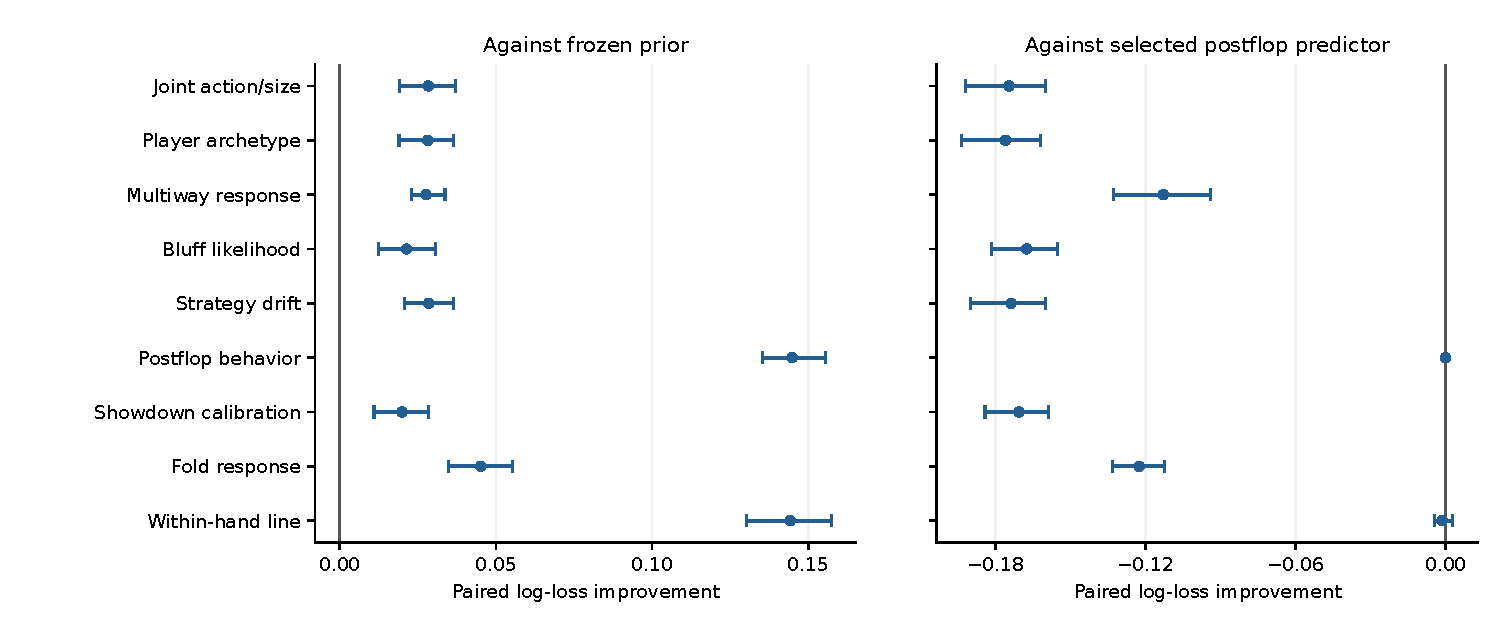
\includegraphics[width=\textwidth]{figures/layer_comparisons.pdf}
\caption{Paired log-loss improvements on component-specific confirmation support. Positive is better. Intervals are the stored whole-game bootstrap intervals with per-comparison \(\alpha=0.05/9\). Support can differ between panels.}
\label{fig:layers}
\end{figure}

\subsection{Range and player-history diagnostics}
The holding-conditioned action-likelihood model scores 17,236 rows from 23 games: log loss is 0.5442, with improvement 0.2840 and a whole-game lower bound of 0.2667. The observed action/size response model scores 98,134 rows: log loss is 0.9969 and improvement is 0.0192, but its lower bound is \(-0.0034\). Its positive mean therefore does not establish a reliable improvement in that metric.

On the fixed sample of 184 revealed holdings, the full range diagnostic has log loss 6.5865, compared with 7.0935 for uniform, 6.7274 for population-only, and 6.7396 with the current-hand likelihood disabled. The stale-profile control is slightly better at 6.5741. Wrong/shuffled-profile controls cover only 66/69 rows, respectively, and are not interchangeable with the full-sample comparisons.

\begin{figure}[htbp]
\centering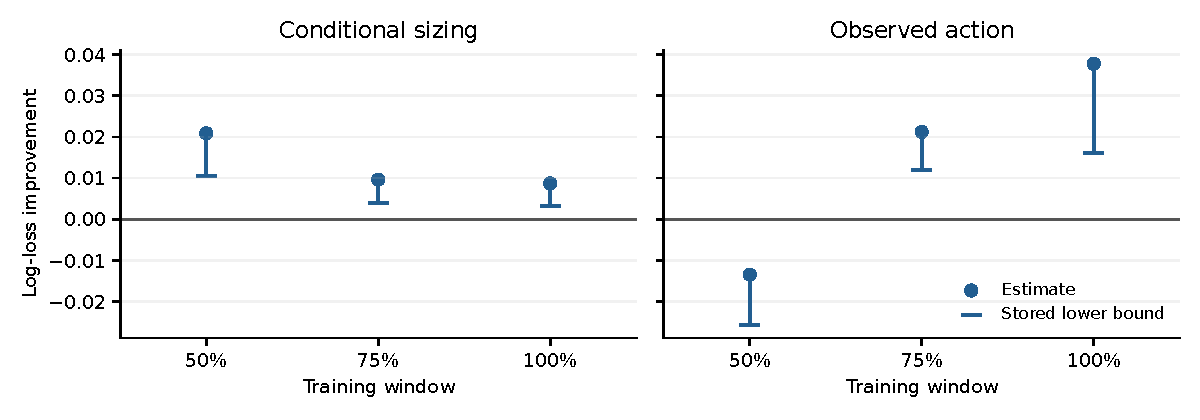
\includegraphics[width=0.85\textwidth]{figures/history_ablations.pdf}
\caption{Session-history versus player-history log-loss improvement in three training windows. Conditional-sizing gains are consistently positive; observed-action gains vary. Points and lower bounds are descriptive results on reused development games.}
\label{fig:history}
\end{figure}

Session history improves conditional sizing over player history in all three windows (Figure~\ref{fig:history}). Observed-action prediction worsens at 50\% and improves at 75\% and 100\%; the 75\% Brier lower bound still crosses zero. Population history also worsens observed-action prediction relative to public-only in all three windows. Player statistics are therefore useful in some measured roles, but their benefit is not universal.

\subsection{Decision value and recorded winnings}
The accepted terminal-value diagnostic contains 465 records, all held and none supported. Missing independent payoff contracts and unproved terminal closure are major reasons. Consequently, it yields no identified off-policy return estimate.

The separate cash-flow audit identifies 4,198 ID-bound candidate hands and reconciles 3,472 across 30 games. This selected subset totals \(+2{,}667.17\) BB: 398 hands have positive net returns, 1,660 negative returns, and 1,414 zero returns. A positive-net-hand count is not the same as pots won, and zero-return records can include nonparticipation. The remaining 726 hands are excluded; exclusion reasons overlap.

The broader StackHUD audit matches 33 inventory games and 5,097 Hero hands. One game is absent; one matched game is excluded because its ledger is unbalanced and flagged for possible omitted nit escrow. The remaining 32 games contain 4,880 hands and complete-game net returns of +486.37 BB over the corrected 66.49 playing hours, yielding \textbf{+7.31 BB/hour}. Two tables changed blinds only outside Hero's hands, so their participation-level stakes remain unambiguous. This complete-game ledger analysis is the primary winnings summary. Its total must not be combined with the selected capture result.

Dividing +486.37 BB by 66.49 hours gives +7.31 BB/hour. The excluded ledger reports \(-163.94\) BB; including it changes both the cohort and the required exposure denominator, so we do not compute an expanded-cohort rate from the 66.49-hour total. Without revised game-level times, a corrected hourly-rate confidence interval cannot be estimated. The observed mean is positive, but this sample does not establish a reliably positive long-run rate. The games span changing runtime versions and do not supply an untreated control or verified recommendation adherence. The result measures recorded gameplay associated with the project, not the Assistant's causal contribution.

\begin{figure}[htbp]
\centering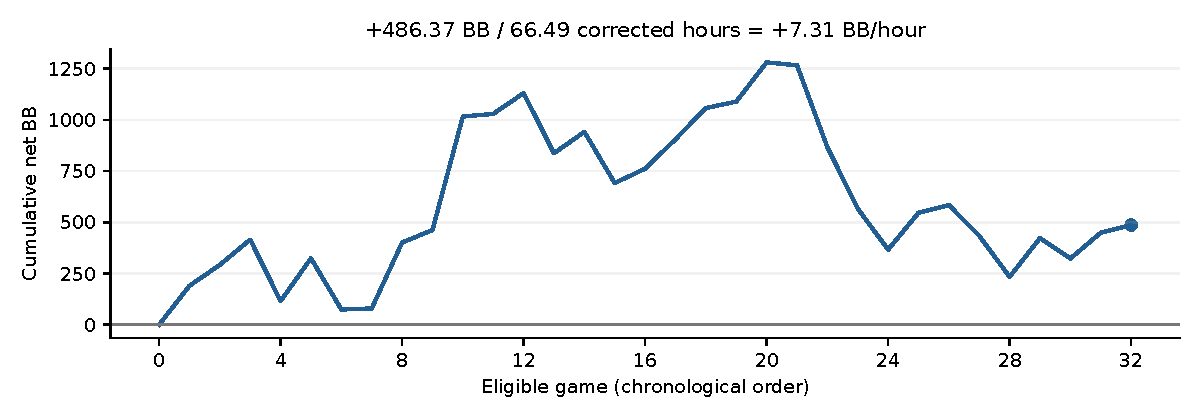
\includegraphics[width=0.88\textwidth]{figures/win_rate.pdf}
\caption{Cumulative complete-game ledger return across 32 eligible games in chronological order. The overall +7.31 BB/hour uses the corrected aggregate duration of 66.49 hours; game-level corrected durations are unavailable. This is not a causal learning curve.}
\label{fig:winrate}
\end{figure}

\section{Limitations}
\paragraph{Computation and resource limits.}
Solver cost grows with private-card combinations, public branches, betting actions, information sets, and independent training/evaluation lanes. We therefore train restricted roots offline and serve compiled policies. The approximate-root default budget is \(64\times60{,}000\) iterations (3.84 million per lane), with checkpoints every 250,000 iterations and identity-checked resume. This is a configured budget, not a claim that every lane consumed it. For the four retained lanes of illustrative root S1-RV-0001, training records show 960,000 iterations and 298,125--298,167 information-set nodes per lane, with qualified early stopping. No total solver wall-time, GPU-hour, or cost estimate is recoverable from these receipts.

We used parallelized workers on the G4 runtime, with concurrency bounded by the host's available logical CPU cores. Offline training and compiled policies reduced live computational requirements.

Our strongest evidence concerns prediction under recorded support conditions and documented changes to experimental advice. Revealed-card selection, repeated use of development games, correlated decisions, limited independent game counts, and distribution changes limit generalization. Solver-root acceptance, source-code tests, artifact installation, predictive improvement, and profitable live play are separate claims. Version-specific recommendation changes cannot be converted into a causal winnings estimate without adherence and outcome controls.

\section{Conclusion}
Poker Assistant integrates solver-derived references, deterministic state/legal checks, bounded sizing, and player-aware models into a working advisory system. Historical Testing logs confirm that selected learned layers changed experimental recommendations; the later runtime retained them as diagnostics pending calibrated strategy development. The empirical results show gains over simple predictive priors and benefits of session history for conditional sizing, but additional layers do not automatically improve on the selected postflop predictor. Verified game ledgers and the corrected aggregate playing-time estimate give +7.31 BB/hour; the duration correction is not independently verified and supports no revised game-level uncertainty interval. Establishing an improvement attributable to the Assistant requires frozen versions, recorded adherence, and a prospective comparison.

\bibliographystyle{plainnat}
\begingroup\small
\bibliography{references}
\endgroup
\appendix
\section{Additional Methods}\label{app:methods}
\subsection{Feature construction and support}
The nine layers predict observed actions with different feature sets. Support checks decide when their outputs may be interpreted; training-time imputation does not create missing historical evidence. The postflop layer uses 61 public-state features. Within-hand surprise adds 63 action-prefix features and requires at least one preceding action. Joint action/size surprise summarizes prior frequencies and aggressive-size moments, requiring at least two completed hands, four decisions, and two aggressive sizes.

Player archetype uses prior action, aggression, fold-response, and sizing rates. For player \(p\), an action rate is shrunk toward the prior population rate:
\begin{equation}
\widetilde p_p(a)=\frac{n_{p,a}+12p_{\rm pop}(a)}{N_p+12}.
\end{equation}
Population statistics also use only earlier completed hands; absent population history gives a uniform action prior. Player support requires two prior hands. Multiway response requires an unambiguously identified target, two prior multiway hands, and four decisions. Ambiguous targets do not become an average over arbitrary opponents.

Strategy drift compares the latest eight completed hands with the preceding 64, using action-rate differences and total variation \(\tfrac12\sum_a|p_{\rm recent}(a)-p_{\rm reference}(a)|\). At least four recent and eight reference hands are required. Fold-response features require a known target and at least four historical facing-size events. A candidate size \(s\), expressed as a pot fraction, must lie inside observed size support; a local fold rate uses at least three events within bandwidth \(\max(0.15,0.25s)\). This is an observational association, not a response to an experimentally assigned size.

Bluff and showdown features use revealed-card evidence stratified by terminal street and aggression. A stratum requires at least two opportunities and one reveal/label; supported strata are opportunity-weighted, with at least three labels and 50\% coverage overall. Bluff labels include losing river aggression, missed draws, and bottom-pair proxies; they do not identify the player's hidden intent. Of 114,605 exact-label rows, 78,465 are accepted. There are also 107,228 fully revealed player-hands; this is a different denominator. Hidden, mucked, or otherwise unavailable holdings are not invented. Reveal selection and conflicting/incomplete evidence limit these layers.

The separate range-likelihood model combines public-state features with enumerated candidate-holding features. A later reveal may supply a training label, but is not exposed as a live feature at the earlier decision. In the hierarchical-history experiment, population, player, and session distributions use
\begin{equation}
p_{\ell}(a\mid x)=\frac{n_{\ell,a}(x)+100p_{\ell-1}(a\mid x)}{N_{\ell}(x)+100}.
\end{equation}
Contexts include stack-depth bands below 150, 150--200, 200--250, and above 250 BB, heads-up versus multiway status, and action family for conditional sizing. The global legal-action prior starts uniformly, with total prior mass equal to the number of legal actions.

\subsection{Fitting, calibration, and evaluation}
Table~\ref{tab:training} gives the installed refit settings. Eight layers fit 2,220,233 rows and calibrate on 113,228; postflop uses its 886,821/47,426-row subset. Feature count and support differ even where fit-row totals coincide.

\begin{table}[!htbp]
\centering\small
\caption{Installed refits. Steps are retained boosting iterations or trees for Extra Trees. Time is the receipt elapsed time for each job, not additive wall-time or total project compute.}
\label{tab:training}
\begin{tabular}{llrrrr}
\toprule
Layer & Family & Features & Steps & $T$ & Seconds \\
\midrule
Joint action/size & LightGBM & 16 & 112 & 0.9 & 108 \\
Player archetype & XGBoost & 15 & 171 & 0.9 & 206 \\
Multiway response & CatBoost & 11 & 357 & 1.0 & 488 \\
Bluff likelihood & XGBoost & 21 & 133 & 1.0 & 189 \\
Strategy drift & CatBoost & 24 & 252 & 1.0 & 433 \\
Postflop behavior & LightGBM & 61 & 453 & 1.0 & 223 \\
Showdown calibration & CatBoost & 9 & 480 & 1.0 & 1,193 \\
Fold response & Extra Trees & 9 & 192 & 1.0 & 389 \\
Within-hand line & CatBoost & 124 & 4,181 & 1.0 & 17,086 \\
\bottomrule
\end{tabular}
\end{table}


For temperature \(T\), legal-action probabilities are proportional to \(p(a\mid x)^{1/T}\), with illegal actions masked and the remainder renormalized. The seven grid-search receipts use \(T\in\{0.5,0.67,0.8,0.9,1,1.1,1.25,1.5,2\}\); the two diagnostic-only receipts retain their inner-fold value. No outer-test loss selects a temperature. For a paired model comparison, bootstrap draw weights \(w_g\) count resampled games, giving
\begin{equation}
\Delta^*=\frac{\sum_g w_g\sum_{j\in g}(\ell_{\rm comparator,j}-\ell_{\rm model,j})}{\sum_g w_g n_g}.
\end{equation}
Thus games are the resampling unit while supported decisions determine the loss average. The winnings point estimate divides total game BB returns by the corrected aggregate hours; no corrected per-game exposure is available for an hourly-rate bootstrap.

\subsection{Solver ranges, evaluation, and compute evidence}
For a legal two-card combination \(c\) and public root state \(x\), range weights combine the declared family, public hand class, action-history/position multipliers, and any declared target-class bias. A strength proxy combines 70\% normalized made-hand category with 30\% normalized preflop class score. Linear and value-heavy families favor stronger holdings; bluff-heavy favors weak holdings and draws; capped favors middle strength; uncapped preserves strong/draw weight; polarized favors extremes; merged combines strong and middle weight. Equilibrium-like has a neutral family multiplier of one, not a claim of Nash calibration. Positive weights have a floor of \(10^{-15}\) before normalization. Joint sampling respects both players' blockers:
\begin{equation}
P(c_0,c_1\mid x)\propto w_0(c_0\mid x)w_1(c_1\mid x)
\mathbf1\{c_0\cap c_1=\varnothing\}.
\end{equation}
Board conflicts are removed before sampling. Conditioning on compatibility can change the marginal distributions; it is not independent sampling followed by ignoring collisions. Strategy keys expose own cards and public state, not the opponent's private cards.

The selected corrected roots comprise uncapped (10), capped (13), linear (6), merged (7), polarized (11), value-heavy (8), bluff-heavy (5), and equilibrium-like (7) families. Their stack anchors contain 17, 18, 14, and 18 roots at 20, 60, 100, and 150 BB, respectively. Restricted-exact lanes use 256 terminal iterations and four private combinations per player. Approximate budgets permit tiers 16 through 128 in increments of 16; qualification may stop a lane before its requested budget.

The 14 behavioral evaluation families are balanced control, uniform legal, tight/loose passive, tight/loose aggressive, overfold, underfold, overcall, underbluff, overbluff, small-size-heavy, large-size-heavy, and jam-heavy. Safe controls are uniform legal, fold/call control, and low-variance control. Four panels, both seat assignments, and 15 candidate-member pairings test a different dimension from private-card range coverage. Exact best-response checks apply only to the restricted exact trees; approximate-root checks do not establish unrestricted exploitability.



\end{document}
